\documentclass{article}
\usepackage[utf8]{inputenc}
\usepackage[english, ukrainian]{babel}
\usepackage{fontsize}
\usepackage{geometry}
\usepackage{amsthm}
\usepackage{amsfonts}
\usepackage{graphicx}
\usepackage[ruled]{algorithm2e}
\usepackage{hyperref}
\usepackage{biblatex}
\usepackage{csquotes}
\usepackage{mathtools}
\usepackage{amsmath}
\usepackage{amssymb}
\usepackage{bbm}
\usepackage{tabularx}
\usepackage{xcolor}

\usepackage{tikz}
\usetikzlibrary{decorations.pathmorphing}

\usepackage{enumitem}
\usepackage{nicefrac}

\usepackage{listings}
\definecolor{codegreen}{rgb}{0,0.6,0}
\definecolor{codegray}{rgb}{0.5,0.5,0.5}
\definecolor{codepurple}{rgb}{0.58,0,0.82}
\definecolor{backcolour}{rgb}{0.95,0.95,0.92}

\lstdefinestyle{mystyle}{
    backgroundcolor=\color{backcolour},   
    commentstyle=\color{codegreen},
    keywordstyle=\color{magenta},
    numberstyle=\tiny\color{codegray},
    stringstyle=\color{codepurple},
    basicstyle=\ttfamily\footnotesize,
    breakatwhitespace=false,         
    breaklines=true,                 
    captionpos=b,                    
    keepspaces=true,                 
    numbers=left,                    
    numbersep=5pt,                  
    showspaces=false,                
    showstringspaces=false,
    showtabs=false,                  
    tabsize=2
}

\lstset{style=mystyle}
\hypersetup{colorlinks=true, linkcolor=[RGB]{255, 3, 209}, citecolor={black}}

\graphicspath{ {../Images/} }

\begin{document}
    \begin{titlepage}
        \begin{center}
            \begin{center}
                НАЦІОНАЛЬНИЙ ТЕХНІЧНИЙ УНІВЕРСИТЕТ УКРАЇНИ
                «КИЇВСЬКИЙ ПОЛІТЕХНІЧНИЙ ІНСТИТУТ імені Ігоря СІКОРСЬКОГО»

                Фізико-технічний інститут
            \end{center}
        $\newline$
        \vspace{3.3cm}
        
        {
        РОЗРАХУНКОВО-ГРАФІЧНА РОБОТА
        
        з кредитного модуля «Методи обчислень»
        
        на тему:
        
        «ОБЧИСЛЮВАЛЬНЕ РОЗВ’ЯЗАННЯ ДИФЕРЕНЦІАЛЬНИХ
        
        РІВНЯНЬ У ЧАСТИННИХ ПОХІДНИХ»
        
        Варіант №10
        }
        \vspace{3cm}
        \begin{flushright}
            Виконав\\студент 3 курсу ФТІ\\групи ФІ-21\\Климентьєв Максим Андрійович
            
            \vspace{1cm}

            Перевірив:\\\underline{\hspace{5cm}}\\Оцінка:\\\underline{\hspace{5cm}}
        \end{flushright}
        \vspace{3.5cm}
        Київ --- 2025
        \end{center}
    \end{titlepage}
    \newpage

    \pagenumbering{gobble}
    \tableofcontents
    \cleardoublepage
    \pagenumbering{arabic}
    \setcounter{page}{3}

    \newpage
    \section{ПОСТАНОВКА ЗАДАЧІ}
    \textbf{Варіант 10}

    Знайти чисельний розв’язок рівняння коливань струни:

    $$ \frac{\partial^2{u}}{\partial{t^2}} = \frac{\partial^2{u}}{\partial{x^2}} + F(t, x) $$
    $$ 0 < x < L = 1 $$
    $$ u(t = 0) = u_0 = x \cdot (x+1) $$
    $$ \frac{\partial{u}}{\partial{t}}(t = 0) = 0 $$
    $$ u(t, 0) = u_1(t) $$
    $$ u(t, L) = u_2(t) $$

    \hrule

    $$ u(t,x) = u_0(x) \cdot \cos(\pi \cdot t) $$
    $$ u_0(x) = u_0 = x \cdot (x+1) $$
    $$ u(t,x) = x \cdot (x+1) \cdot \cos(\pi \cdot t) $$

    \hrule

    $$ u(t,0) = 0 \cdot 1 \cdot \cos(\pi \cdot t) = 0 $$
    $$ u(t, L) = L \cdot (L+1) \cdot \cos(\pi \cdot t) = 1 \cdot 2 \cdot \cos(\pi \cdot t) = 2 \cdot \cos(\pi \cdot t) $$

    \hrule

    $$ \frac{\partial{u}}{\partial{x}} = 2 \cdot x \cdot \cos(\pi \cdot t) + \cos(\pi \cdot t) $$
    $$ \frac{\partial^2{u}}{\partial{x^2}} = 2 \cdot \cos(\pi \cdot t) $$

    $$ \frac{\partial{u}}{\partial{t}} = -\pi \cdot x \cdot (x+1) \cdot \sin(\pi \cdot t) $$
    % $$ \frac{\partial{u}}{\partial{t}} = -\pi \cdot x \cdot (x+1) \cdot \sin(\pi \cdot t) $$
    $$ \frac{\partial^2{u}}{\partial{t^2}} = -\pi^2 \cdot x \cdot (x+1) \cdot \cos(\pi \cdot t) $$

    \hrule

    $$ \frac{\partial^2{u}}{\partial{t^2}} = \frac{\partial^2{u}}{\partial{x^2}} + F(t, x) $$
    $$ \frac{\partial^2{u}}{\partial{t^2}} - \frac{\partial^2{u}}{\partial{x^2}} = F(t, x) $$
    $$ F(t, x) = -\pi^2 \cdot x \cdot (x+1) \cdot \cos(\pi \cdot t) - 2 \cdot \cos(\pi \cdot t) $$
    $$ F(t, x) = -\cos(\pi \cdot t) \cdot \left(\pi^2 \cdot x \cdot (x+1) + 2\right) $$

    \hrule

    Рівняння --- гіперболічного типу.
    
    Є нелінійність - будемо робити через явну схему.

    \hrule

    Навести приклади процесів, які моделюються за допомогою диференціальних рівнянь у частинних похідних гіперболічного типу
    
    \newpage
    \section{ОГЛЯД ТА АНАЛІЗ ІСНУЮЧИХ МЕТОДІВ ЧИСЕЛЬНОГО РОЗВ’ЯЗАННЯ ДРЧП}
        \subsection{Тришарова схема з вагами}
            \label{enum:main}
            \begin{align*}
                - \frac{\Delta{t}^2 \cdot \sigma_1}{\Delta{x}^2} \cdot u(k+1, i-1) & + \left( 1 + 2 \cdot \frac{\Delta{t}^2 \cdot \sigma_1}{\Delta{x}^2} \right) \cdot u(k+1, i) - \frac{\Delta{t}^2 \cdot \sigma_1}{\Delta{x}^2} \cdot u(k+1, i+1) = \\
                & = 2 \cdot u(k, i) - u(k-1, i)  + \\
                & + \Delta{t}^2 \cdot \sigma_1 \cdot F(k+1, i) + \\
                & + \Delta{t}^2 \cdot \left(1 - \sigma_1 - \sigma_2 \right) \cdot \left(\frac{u(k, i+1) - 2 \cdot u(k, i) + u(k, i-1)}{\Delta{x}^2} + F(k, i)\right) + \\
                & + \Delta{t}^2 \cdot \sigma_2 \cdot \left(\frac{u(k-1, i+1) - 2 \cdot u(k-1, i) + u(k-1, i-1)}{\Delta{x}^2} + F(k-1, i)\right)
            \end{align*}

            Приведення до такого виду \eqref{subsec:main}

            Після чого вирішується така система кожну ітерацію:
            $$ Ax = B $$ де х - незалежна змінна для u, де B - права частина, порахована через минулі незалежні змінні, де A - тридіагональна матриця з коефіціентів,  
            $$ Shape (nx - 2, nx - 2) = A$$ 
            $$ Shape (nx - 2) = B$$
            $$ Shape (nx - 2) = x$$

            Приведення до такого виду \eqref{subsec:equation}

            \begin{itemize}
                \item Переваги: Необхідність меншої кількості точок для часу.
                \item Недоліки\label{itemz:main}:
                    \begin{itemize}
                        \item Треба нормально так подумати, аби правильно реалізувати;
                        \item Для коректної роботи схеми: $ \sigma_1 \geq \sigma_2 $;
                        \item $ \sigma_1 + \sigma_2 \geq \frac{1}{2} $ --- схема є \textbf{стійкою} для будь-яких $ \Delta{x} $ та $ \Delta{t} $;
                        \item $ \sigma_1 + \sigma_2 < \frac{1}{2} $ --- схема є \textbf{умовно стійкою}, тобто вона буде працювати для:
                        $$ \Delta{t} \leq \frac{\Delta{x}}{\sqrt{1 - 2 \cdot(\sigma_1 + \sigma_2)}} $$
                \end{itemize}
            \end{itemize}

        \subsection{Явна схема}
            \label{enum:straight}
            $$ u(k+1, i) = 2 \cdot u(k, i) - u(k-1, i) + \Delta{t}^2 \cdot \left( \frac{u(k, i+1) - 2 \cdot u(k, i) + u(k, i-1)}{\Delta{x}^2} + F(k, i) \right) $$

            Приведення до такого виду \eqref{subsec:straight}

            \begin{itemize}
                \item Переваги: Простота реалізації, висока швидкість
                \item Недоліки\label{itemz:straight}: Необхідна стійкість $ \frac{\Delta{t}}{\Delta{x}^2} \leq 0.5 $
            \end{itemize}

        Оберемо Тришарову схему з вагами \eqref{enum:main}

    \newpage
    \section{ДОСЛІДЖЕННЯ УМОВ ЗАСТОСУВАННЯ ОБРАНОГО МЕТОДУ}

    Як вже згадувалось у недоліках \eqref{enum:main}:

    \begin{itemize}
        \item Для коректної роботи схеми: $ \sigma_1 \geq \sigma_2 $;
        \item $ \sigma_1 + \sigma_2 \geq \frac{1}{2} $ --- схема є \textbf{стійкою} для будь-яких $ \Delta{x} $ та $ \Delta{t} $;
        \item $ \sigma_1 + \sigma_2 < \frac{1}{2} $ --- схема є \textbf{умовно стійкою}, тобто вона буде працювати для:
        $$ \Delta{t} \leq \frac{\Delta{x}}{\sqrt{1 - 2 \cdot(\sigma_1 + \sigma_2)}} $$
    \end{itemize}

    \newpage
    \section{ОПИС ПРОГРАМНОЇ РЕАЛИЗАЦІЇ}
        Параметри:

        Кількість вузлів $ x = 100 $
        
        Кількість індексів дискретного часу $ t = 1000 $
        
        Відстань між сусідніми просторовими вузлами $ \Delta{x} = 0.01 $
        
        Відстань між сусідніми моментами часу $ \Delta{t} = 0.002 $

        $ L = 1 $

        $ T = 2 $

        Застосовано Тришарову схему з вагами \eqref{enum:main}.

        Масиви, початковий та кінцевий \eqref{subsec:xsr}

        Побудовано графіки:

        \begin{figure}[h!]
            \includegraphics[width=0.5\linewidth]{Main_2d.png}
            \includegraphics[width=0.5\linewidth]{Main_3d.png}
            \caption{Поверхня U(t, x) у 2D та 3D}
        \end{figure}

        \begin{figure}[h!]
            \centering
            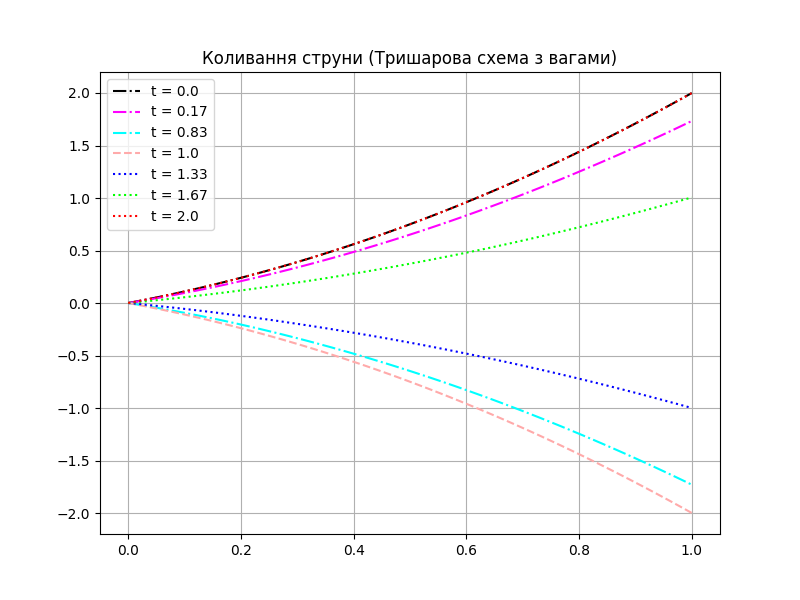
\includegraphics[width=0.5\linewidth]{Main_key_time.png}
            \caption{Зрізи U(t, x) для фіксованих моментів часу}
        \end{figure}

        \begin{figure}[h!]
            \centering
            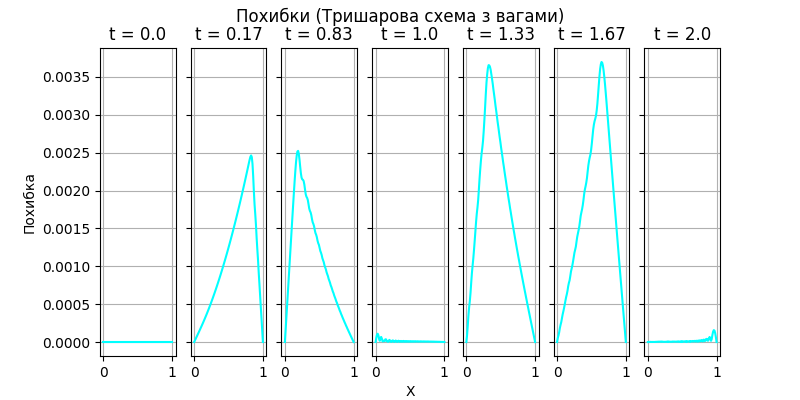
\includegraphics[width=0.5\linewidth]{Main_error.png}
            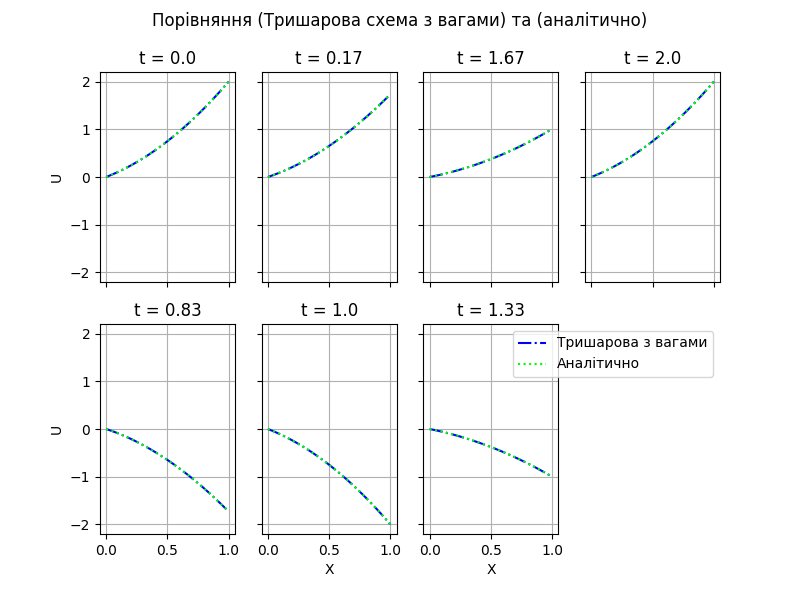
\includegraphics[width=0.5\linewidth]{Main_compare.png}
            \caption{Похибка}
        \end{figure}
    \newpage
    \section{ОГЛЯД МЕТОДІВ ПІДВИЩЕННЯ ТОЧНОСТІ}

        Можна збільшити кількість точок t.

    \newpage
    \section{ЗАСТОСУВАННЯ МЕТОДУ ПІДВИЩЕННЯ ТОЧНОСТІ ТА ЕФЕКТИВНОСТІ РОЗВ’ЯЗКУ ДО ПРИКЛАДУ РОБОТИ}
        Зі збільшенням t зменшується похибка
        \begin{figure}[h!]
            \centering
            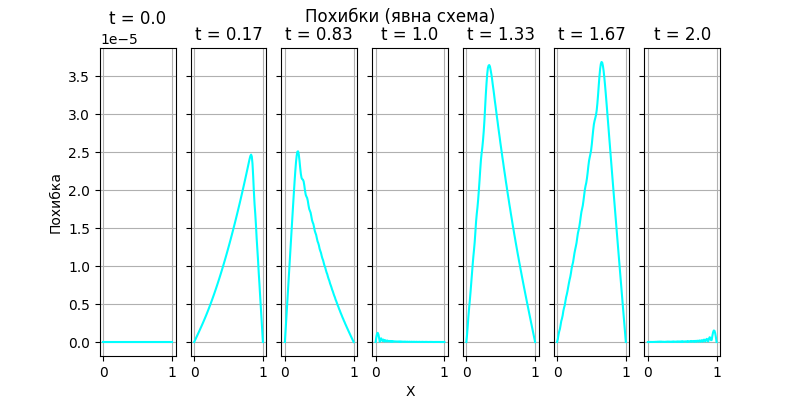
\includegraphics[width=0.5\linewidth]{Straight_error.png}
            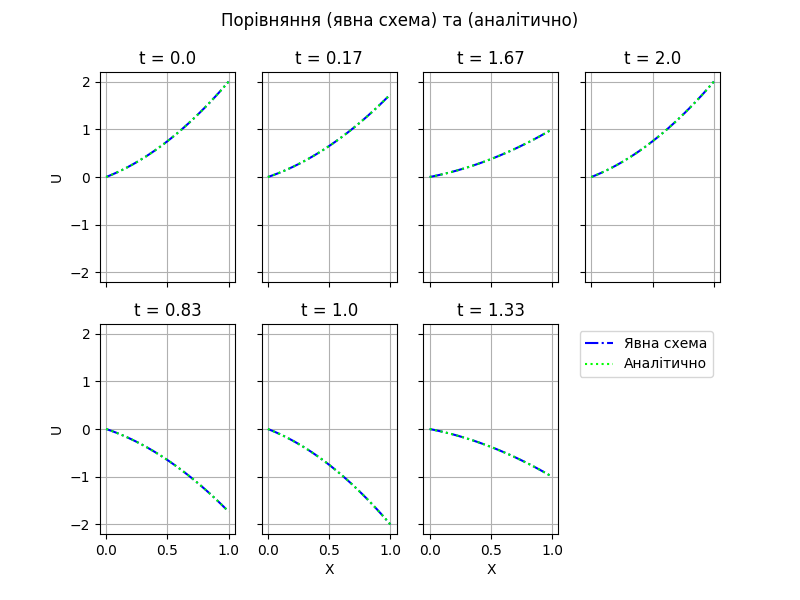
\includegraphics[width=0.5\linewidth]{Straight_compare.png}
            \caption{Похибка (Фотографії узято з явної схеми, оскільки при однаковій кількості точок вони дають однакову похибку)}
        \end{figure}
    \newpage
    \section{ВИСНОВКИ}
        Застосувавши Тришарову схему з вагами ми отримали коливання струни, яке майже таке ж, як аналітичний розв'язок.
        Приклади процесів, які моделюються за допомогою гіперболічних диференціальних рівнянь у частинних похідних:
        \begin{itemize}
            \item Коливання струни. Одне з таких можна побачити вище, у постановці задачі.
            \item Коливання мембрани. Таке ж, як коливання струни, але з двома незалежними змінними.
            \item Поширення звукових хвиль.
            \item Поширення електромагнітних хвиль.
        \end{itemize}
    \newpage
    \section{СПИСОК ВИКОРИСТАНИХ ДЖЕРЕЛ}
    \begin{enumerate}
        \item Методи обчислень: Розрахунково-графічна робота [Електронний ресурс]:
            навч. посіб. для студ. спец. 113 «Прикладна математика» / КПІ ім. Ігоря
            Сікорського; уклад.: І.В. Стьопочкіна. – Електронні текстові дані (1 файл: 7,7
            Мбайт). – Київ : КПІ ім. Ігоря Сікорського, 2022. – 56 с.
        \item W. T. Lee.
            Tridiagonal Matrices: Thomas Algorithm. 
            MS6021, Scientific Computation, University of Limerick.
            URL: \url{http://www.industrial-maths.com/ms6021_thomas.pdf}
    \end{enumerate}
    \newpage
    \section{ДОДАТКИ}
        \subsection{Масиви, початковий та кінцевий}
            \label{subsec:xsr}

            Початкова матриця (1000x100): 
            $$
            \left(
                \begin{matrix}
                    0.0 & 0.01020304050607081 & 0.020610141822263034 & $\dots$ & 1.9697990001020307 & 2.0 \\
                    0.0 & 0.01020304050607081 & 0.020610141822263034 & $\dots$ & 1.9697990001020307 & 1.9999604426373665 \\
                    0.0 & 0.0 & 0.0 & $\dots$ & 0.0 & 1.999841772114251 \\
                    0.0 & 0.0 & 0.0 & $\dots$ & 0.0 & 1.9996439931249463 \\
                    0.0 & 0.0 & 0.0 & $\dots$ & 0.0 & 1.9993671134930677 \\
                    0.0 & 0.0 & 0.0 & $\dots$ & 0.0 & 1.999011144171243 \\
                    0.0 & 0.0 & 0.0 & $\dots$ & 0.0 & 1.99857609924068 \\
                    0.0 & 0.0 & 0.0 & $\dots$ & 0.0 & 1.9980619959106087 \\
                    0.0 & 0.0 & 0.0 & $\dots$ & 0.0 & 1.9974688545176011 \\
                    0.0 & 0.0 & 0.0 & $\dots$ & 0.0 & 1.9967966985247663 \\

                    \dots & \dots & \dots & \dots & \dots & \dots \\

                    0.0 & 0.0 & 0.0 & $\dots$ & 0.0 & 1.999841772114251 \\
                    0.0 & 0.0 & 0.0 & $\dots$ & 0.0 & 1.9999604426373665 \\
                    0.0 & 0.0 & 0.0 & $\dots$ & 0.0 & 2.0 \\

                    \label{mat:xs}
                \end{matrix}
            \right)
            $$
        
            Фінальна матриця (1000x100): 
            $$
            \left(
                \begin{matrix}
                    0.0 & 0.01020304050607081 & 0.020610141822263034 & $\dots$ & 1.9697990001020307 & 2.0 \\
                    0.0 & 0.01020304050607081 & 0.020610141822263034 & $\dots$ & 1.9697990001020307 & 1.9999604426373665 \\
                    0.0 & 0.010202637068360935 & 0.02060932671944144 & $\dots$ & 1.9697195581339106 & 1.999841772114251 \\
                    0.0 & 0.010201830367918184 & 0.020607696720591286 & $\dots$ & 1.9695592711572425 & 1.9996439931249463 \\
                    0.0 & 0.010200620584156602 & 0.020605252064306783 & $\dots$ & 1.969316960781178 & 1.9993671134930677 \\
                    0.0 & 0.01019900789625577 & 0.020601993020245186 & $\dots$ & 1.9689917575962361 & 1.999011144171243 \\
                    0.0 & 0.010196992479686104 & 0.020597919887864045 & $\dots$ & 1.9685831569058483 & 1.99857609924068 \\
                    0.0 & 0.010194574504149699 & 0.020593032994595854 & $\dots$ & 1.9680910411973875 & 1.9980619959106087 \\
                    0.0 & 0.010191754133025591 & 0.020587332693514874 & $\dots$ & 1.9675156681484067 & 1.9974688545176011 \\
                    0.0 & 0.010188531524273675 & 0.020580819360640993 & $\dots$ & 1.9668576264838946 & 1.9967966985247663 \\

                    \dots & \dots & \dots & \dots & \dots & \dots \\

                    0.0 & 0.01020677415746861 & 0.020603325625168555 & $\dots$ & 1.9695620769242572 & 1.999841772114251 \\
                    0.0 & 0.010206447367528225 & 0.020606105713839022 & $\dots$ & 1.969687107685745 & 1.9999604426373665 \\
                    0.0 & 0.010205302713256682 & 0.02060844158171087 & $\dots$ & 1.9697346596870817 & 2.0 \\

                    \label{mat:xr}
                \end{matrix}
            \right)
            $$


        \subsection{Тришарова схема з вагами}
            \label{subsec:main}
            $$ u(t, x) $$
            $$ \frac{\partial^2{u}}{\partial{t^2}} = \frac{\partial^2{u}}{\partial{x^2}} + F(t, x) $$
            
            \begin{align*}
                \frac{u_i^{k+1} - 2 \cdot u_i^{k} + u_i^{k-1}}{\Delta{t}^2}& = \sigma_1 \cdot \left(\frac{u_{i+1}^{k+1} - 2 \cdot u_i^{k+1} + u_{i-1}^{k+1}}{\Delta{x}^2} + F_i^{k+1}\right) + \\
                & + \left(1 - \sigma_1 - \sigma_2 \right) \cdot \left(\frac{u_{i+1}^{k} - 2 \cdot u_i^{k} + u_{i-1}^{k}}{\Delta{x}^2} + F_i^{k}\right) + \\
                & + \sigma_2 \cdot \left(\frac{u_{i+1}^{k-1} - 2 \cdot u_i^{k-1} + u_{i-1}^{k-1}}{\Delta{x}^2} + F_i^{k-1}\right)
            \end{align*}
            
            \begin{align*}
                u_i^{k+1} & = 2 \cdot u_i^{k} - u_i^{k-1} + \Delta{t}^2 \cdot \sigma_1 \cdot \left(\frac{u_{i+1}^{k+1} - 2 \cdot u_i^{k+1} + u_{i-1}^{k+1}}{\Delta{x}^2} + F_i^{k+1}\right) + \\
                & + \Delta{t}^2 \cdot \left(1 - \sigma_1 - \sigma_2 \right) \cdot \left(\frac{u_{i+1}^{k} - 2 \cdot u_i^{k} + u_{i-1}^{k}}{\Delta{x}^2} + F_i^{k}\right) + \\
                & + \Delta{t}^2 \cdot \sigma_2 \cdot \left(\frac{u_{i+1}^{k-1} - 2 \cdot u_i^{k-1} + u_{i-1}^{k-1}}{\Delta{x}^2} + F_i^{k-1}\right)
            \end{align*}
            
            \begin{align*}
                u_i^{k+1} & - \frac{\Delta{t}^2 \cdot \sigma_1}{\Delta{x}^2} \cdot \left(u_{i+1}^{k+1} - 2 \cdot u_i^{k+1} + u_{i-1}^{k+1}\right) = \\
                & = 2 \cdot u_i^{k} - u_i^{k-1}  + \\
                & + \Delta{t}^2 \cdot \sigma_1 \cdot F_i^{k+1} + \\
                & + \Delta{t}^2 \cdot \left(1 - \sigma_1 - \sigma_2 \right) \cdot \left(\frac{u_{i+1}^{k} - 2 \cdot u_i^{k} + u_{i-1}^{k}}{\Delta{x}^2} + F_i^{k}\right) + \\
                & + \Delta{t}^2 \cdot \sigma_2 \cdot \left(\frac{u_{i+1}^{k-1} - 2 \cdot u_i^{k-1} + u_{i-1}^{k-1}}{\Delta{x}^2} + F_i^{k-1}\right)
            \end{align*}

            \begin{align*}
                u(k+1, i) & - \frac{\Delta{t}^2 \cdot \sigma_1}{\Delta{x}^2} \cdot \left(u(k+1, i+1) - 2 \cdot u(k+1, i) + u(k+1, i-1)\right) = \\
                & = 2 \cdot u(k, i) - u(k-1, i)  + \\
                & + \Delta{t}^2 \cdot \sigma_1 \cdot F(k+1, i) + \\
                & + \Delta{t}^2 \cdot \left(1 - \sigma_1 - \sigma_2 \right) \cdot \left(\frac{u(k, i+1) - 2 \cdot u(k, i) + u(k, i-1)}{\Delta{x}^2} + F(k, i)\right) + \\
                & + \Delta{t}^2 \cdot \sigma_2 \cdot \left(\frac{u(k-1, i+1) - 2 \cdot u(k-1, i) + u(k-1, i-1)}{\Delta{x}^2} + F(k-1, i)\right)
            \end{align*}

        \subsection{Явна схема}
            \label{subsec:straight}
            $$ u(t, x) $$
            $$ \frac{\partial^2{u}}{\partial{t^2}} = \frac{\partial^2{u}}{\partial{x^2}} + F(t, x) $$
            $$ \frac{u_i^{k+1} - 2 \cdot u_i^{k} + u_i^{k-1}}{\Delta{t}^2} = \frac{u_{i+1}^{k} - 2 \cdot u_i^{k} + u_{i-1}^{k}}{\Delta{x}^2} + F_i^{k} $$
            $$ u_i^{k+1} - 2 \cdot u_i^{k} + u_i^{k-1} = \Delta{t}^2 \cdot \left( \frac{u_{i+1}^{k} - 2 \cdot u_i^{k} + u_{i-1}^{k}}{\Delta{x}^2} + F_i^{k} \right) $$
            $$ u_i^{k+1} = 2 \cdot u_i^{k} - u_i^{k-1} + \Delta{t}^2 \cdot \left( \frac{u_{i+1}^{k} - 2 \cdot u_i^{k} + u_{i-1}^{k}}{\Delta{x}^2} + F_i^{k} \right) $$

        \subsection{Ax = B}
            \label{subsec:equation}
            A = 
            $$\left(
                \begin{matrix}
                    \left( 1 + 2 \cdot \frac{\Delta{t}^2 \cdot \sigma_1}{\Delta{x}^2} \right) & - \frac{\Delta{t}^2 \cdot \sigma_1}{\Delta{x}^2} & 0.0 & \dots & 0.0 & 0.0 & 0.0 \\
                    - \frac{\Delta{t}^2 \cdot \sigma_1}{\Delta{x}^2} & \left( 1 + 2 \cdot \frac{\Delta{t}^2 \cdot \sigma_1}{\Delta{x}^2} \right) & - \frac{\Delta{t}^2 \cdot \sigma_1}{\Delta{x}^2} & \dots & 0.0 & 0.0 & 0.0 \\
                    0.0 & - \frac{\Delta{t}^2 \cdot \sigma_1}{\Delta{x}^2} & \left( 1 + 2 \cdot \frac{\Delta{t}^2 \cdot \sigma_1}{\Delta{x}^2} \right) & \dots & 0.0 & 0.0 & 0.0 \\
                    0.0 & 0.0 & - \frac{\Delta{t}^2 \cdot \sigma_1}{\Delta{x}^2} & \dots & 0.0 & 0.0 & 0.0 \\
                    0.0 & 0.0 & 0.0 & \dots & 0.0 & 0.0 & 0.0 \\
                    0.0 & 0.0 & 0.0 & \dots & 0.0 & 0.0 & 0.0 \\
                    0.0 & 0.0 & 0.0 & \dots & 0.0 & 0.0 & 0.0 \\
                    0.0 & 0.0 & 0.0 & \dots & 0.0 & 0.0 & 0.0 \\
                    0.0 & 0.0 & 0.0 & \dots & 0.0 & 0.0 & 0.0 \\
                    0.0 & 0.0 & 0.0 & \dots & 0.0 & 0.0 & 0.0 \\

                    \dots & \dots & \dots & \dots & \dots \\

                    0.0 & 0.0 & 0.0 & \dots & \left( 1 + 2 \cdot \frac{\Delta{t}^2 \cdot \sigma_1}{\Delta{x}^2} \right) & - \frac{\Delta{t}^2 \cdot \sigma_1}{\Delta{x}^2} & 0.0 \\
                    0.0 & 0.0 & 0.0 & \dots & - \frac{\Delta{t}^2 \cdot \sigma_1}{\Delta{x}^2} & \left( 1 + 2 \cdot \frac{\Delta{t}^2 \cdot \sigma_1}{\Delta{x}^2} \right) & - \frac{\Delta{t}^2 \cdot \sigma_1}{\Delta{x}^2} \\
                    0.0 & 0.0 & 0.0 & \dots & 0.0 & - \frac{\Delta{t}^2 \cdot \sigma_1}{\Delta{x}^2} & \left( 1 + 2 \cdot \frac{\Delta{t}^2 \cdot \sigma_1}{\Delta{x}^2} \right) \\
                \end{matrix}
            \right)$$
            B = 
            $$
            \left(
                \begin{matrix}
                    2 \cdot u(k, 1) - u(k-1, 1)  + \\
                     + \Delta{t}^2 \cdot \sigma_1 \cdot F(k+1, 1) + \\
                     + \Delta{t}^2 \cdot \left(1 - \sigma_1 - \sigma_2 \right) \cdot \left(\frac{u(k, 2) - 2 \cdot u(k, 1) + u(k, 0)}{\Delta{x}^2} + F(k, 1)\right) + \\
                     + \Delta{t}^2 \cdot \sigma_2 \cdot \left(\frac{u(k-1, 2) - 2 \cdot u(k-1, 1) + u(k-1, 0)}{\Delta{x}^2} + F(k-1, 1)\right) + \\
                     + \frac{\Delta{t}^2 \cdot \sigma_1}{\Delta{x}^2} \cdot u(k+1, 0) \\
                    \\

                    2 \cdot u(k, 2) - u(k-1, 2)  + \\
                     + \Delta{t}^2 \cdot \sigma_1 \cdot F(k+1, 2) + \\
                     + \Delta{t}^2 \cdot \left(1 - \sigma_1 - \sigma_2 \right) \cdot \left(\frac{u(k, 3) - 2 \cdot u(k, 2) + u(k, 1)}{\Delta{x}^2} + F(k, 2)\right) + \\
                     + \Delta{t}^2 \cdot \sigma_2 \cdot \left(\frac{u(k-1, 3) - 2 \cdot u(k-1, 2) + u(k-1, 1)}{\Delta{x}^2} + F(k-1, 2)\right) \\
                    \\

                    \cdots \\
                    \\

                    2 \cdot u(k, i) - u(k-1, nx - 3) + \\
                     + \Delta{t}^2 \cdot \sigma_1 \cdot F(k+1, nx - 3) + \\
                     + \Delta{t}^2 \cdot \left(1 - \sigma_1 - \sigma_2 \right) \cdot \left(\frac{u(k, nx - 2) - 2 \cdot u(k, nx - 3) + u(k, nx - 4)}{\Delta{x}^2} + F(k, nx - 3)\right) + \\
                     + \Delta{t}^2 \cdot \sigma_2 \cdot \left(\frac{u(k-1, nx - 2) - 2 \cdot u(k-1, nx - 3) + u(k-1, nx - 4)}{\Delta{x}^2} + F(k-1, nx - 3)\right) \\
                    \\

                    2 \cdot u(k, i) - u(k-1, nx - 2) + \\
                     + \Delta{t}^2 \cdot \sigma_1 \cdot F(k+1, nx - 2) + \\
                     + \Delta{t}^2 \cdot \left(1 - \sigma_1 - \sigma_2 \right) \cdot \left(\frac{u(k, nx - 1) - 2 \cdot u(k, nx - 2) + u(k, nx - 3)}{\Delta{x}^2} + F(k, nx - 2)\right) + \\
                     + \Delta{t}^2 \cdot \sigma_2 \cdot \left(\frac{u(k-1, nx - 1) - 2 \cdot u(k-1, nx - 2) + u(k-1, nx - 3)}{\Delta{x}^2} + F(k-1, nx - 2)\right) + \\
                     + \frac{\Delta{t}^2 \cdot \sigma_1}{\Delta{x}^2} \cdot u(k+1, nx - 2) \\
                \end{matrix}
            \right)$$
            x = 
            $$
            \left(
                \begin{matrix}
                    u(k+1, 1) \\
                    \cdots \\
                    u(k+1, nx - 2) \\
                \end{matrix}
            \right)$$

\end{document}